%
%
% Sample document of Finance and Stochastics
\documentclass[fist]{svjour3}          


\usepackage{graphicx}
\usepackage{amssymb,amsfonts,amsmath,amsxtra}


\iffalse %% set to true (preferred), if commercial set of Times is available on your TeX system
%% 
 \usepackage{times}
 \usepackage[LY1]{fontenc}
 \usepackage[LY1,mtbold]{mathtime}
\else
 \usepackage[LY1]{fontenc}
 \usepackage{txfonts}
\fi 


%\showgrid % show baseline grid with linenumers on every page 
\smartqed  % flush right qed marks, e.g. at end of proof


\journalname{Finance and Stochastics}
\begin{document}


\title{Insert your title here%\thanks{%
%Note about the article that should go on the front page should be
%placed here. 
%Grants and acknowledgments should be placed at the end of the article.}
}


\subtitle{Do you have a subtitle?\\ If so, write it here}

\author{\fnm{First}     % Firstname(s)
        \snm{Author}    % Surname 
        \jr{Jr.}%       % Jr.
       \and
        \fnm{Second}    
        \snm{Author}
}

\institute{\inits{F.} \snm{Author} % Initials & Surname
           \at 
           \orgdiv{First Address},        % Organization Division (e.g. Department, Faculty, Lab, D-MATH, etc.)
           \orgname{Organization Name},   % Organization Name (e.g. University, Institute, etc.)
           \street{Street 112},           % Street name and number
           \city{City},                   % City  *Mandatory
           \postcode{Postcode}            % Post code 
           \state{State},                 % State or state code (e.g. Ontario, MA)
           \cny{Country}\\                % Country *Mandatory
           \email{fauthor@example.com}    % Email address
	   % 
         \and
           \inits{S.} \snm{Author}
           \at 
           \orgdiv{},
	   \orgname{},
           \street{},
           \city{},
           \postcode{}
	   \state{}, 
	   \cny{}
	  }
           

% The correct dates will be entered by the editor
\date{\received{date} / \accepted{date}}

\maketitle

\begin{abstract}
Insert your abstract here. Insert your abstract here. Insert your abstract here.
Insert your abstract here. Insert your abstract here. Insert your abstract here.
Insert your abstract here. Insert your abstract here. Insert your abstract here.

\keywords{First keyword \and Second keyword \and More}

%% Please include in your manuscript the MSC 2000 numbers. See http://www.ams.org/msc
\subclass{XXXX \and YYY}

%% Please include the JEL classification codes. See http://www.aeaweb.org/journal/jel_class_system.html
\JEL{XXX \and YYY }
\end{abstract}


\section{Introduction}
\label{intro}
Your text comes here. Separate text sections with
\section{Section title}
\label{sec:1}
Text with citations \cite{RefB} and \cite{RefJ}.
\subsection{Subsection title}
\label{sec:2}
as required. Don't forget to give each section
and subsection a unique label (see Sect.~\ref{sec:1}).
\paragraph{Paragraph headings} Use paragraph headings as needed.
\begin{equation}
a^2+b^2=c^2
\end{equation}

% For one-column wide figures use
\begin{figure}
% Use the relevant command to insert your figure file.
% For example, with the graphicx package use
% 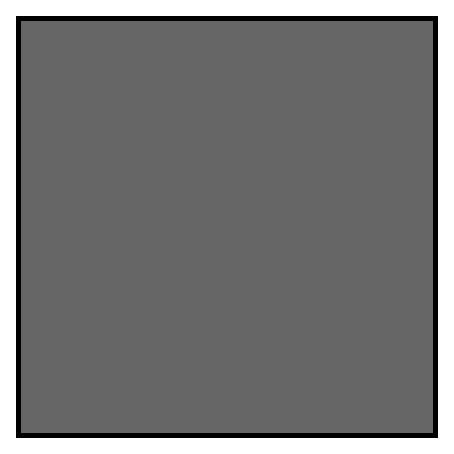
\includegraphics{example.eps}
%
% figure caption is below the figure
\caption{Please write your figure caption here}
\label{fig:1}       % Give a unique label
\end{figure}
%
% For two-column wide figures use
\begin{figure*}
% Use the relevant command to insert your figure file.
% For example, with the graphicx package use
%  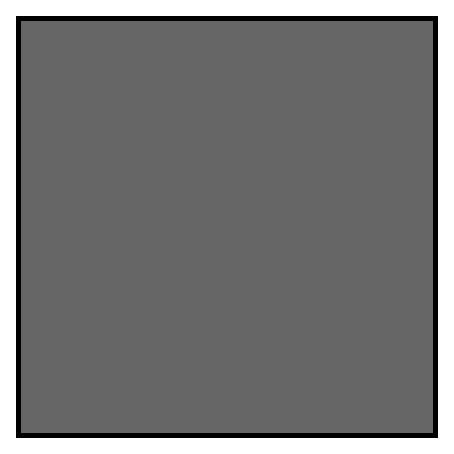
\includegraphics[width=0.75\textwidth]{example.eps}
%
% figure caption is below the figure
\caption{Please write your figure caption here}
\label{fig:2}       % Give a unique label
\end{figure*}
%
% For tables use
\begin{table}
% table caption is above the table
\caption{Please write your table caption here}
\label{tab:1}       % Give a unique label
% For LaTeX tables use
\begin{tabular}{lll}
\hline\noalign{\smallskip}
first & second & third  \\
\noalign{\smallskip}\hline\noalign{\smallskip}
number & number & number \\
number & number & number \\
\noalign{\smallskip}\hline
\end{tabular}
\end{table}


%
% \begin{acknowledgements}
%  If you'd like to thank anyone, place your comments here
%  and remove the percent signs.
%
%  Financial support and grants acknowledgements should be placed here. 
% \end{acknowledgements}
%

% BibTeX users please use one of
%\bibliographystyle{spr-mp}               % MathPhys style, numbered citations
%\bibliographystyle{spr-mp-nameyear}      % MathPhys style, nameyear citations
%\bibliography{}   % name your BibTeX data base
% BibTeX users please use MathPhys style


% Non-BibTeX users please use
\begin{thebibliography}{}
%
% and use \bibitem to create references. Consult the Instructions
% for authors for reference list style.
%
\bibitem{RefJ}
% Format for Journal Reference
Author, Article title, Journal, Volume, page numbers (year)
% Format for books
\bibitem{RefB}
Author, Book title, page numbers. Publisher, place (year)
% etc
\end{thebibliography}



\end{document}
